\section{Amplitudes de CSI (seção 3)}

\subsection{Cálculo}

Em cada linha de cada TXT, a primeira coluna (informação temporal) é separada e os 128 valores restantes são agrupados em 64 pares (imaginária, real), nessa ordem. A amplitude de cada par é |H| = (Re(H)\textsuperscript{2} + Im(H)\textsuperscript{2})\textsuperscript{1/2}, como na função get\_amps de Scripts/CSI.py. Cada TXT gera uma matriz com uma linha por registro e 64 colunas; por exemplo, o arquivo csi\_data\_1722274497.txt (s12, FA, 974 registros) gera uma matriz 974 × 64. As amplitudes foram calculadas para os 30 arquivos selecionados.

\subsection{Verificação numérica do par 20}

{\footnotesize
\begin{longtable}{|>{\centering\arraybackslash}p{4.03cm}|>{\centering\arraybackslash}p{1.45cm}|>{\centering\arraybackslash}p{0.89cm}|>{\centering\arraybackslash}p{2.26cm}|>{\centering\arraybackslash}p{1.93cm}|>{\centering\arraybackslash}p{2.74cm}|}
\caption{Verificação do cálculo da amplitude (gravação s12/FA, ordem\_selecao = 1).}\\
\hline
\textbf{TXT} & \textbf{Linha do TXT} & \textbf{Par} & \textbf{Imaginária (coluna 40)} & \textbf{Real (coluna 41)} & \textbf{Amplitude (coluna 20 da matriz)} \\ \hline
\endfirsthead
\hline
\textbf{TXT} & \textbf{Linha do TXT} & \textbf{Par} & \textbf{Imaginária (coluna 40)} & \textbf{Real (coluna 41)} & \textbf{Amplitude (coluna 20 da matriz)} \\ \hline
\endhead
csi\_data\_1722274497.txt (s12, FA) & 1 & 20 & 33 & 5 & 33,38 \\ \hline
\end{longtable}
}

Conferência: (5\textsuperscript{2} + 33\textsuperscript{2})\textsuperscript{1/2} = 1114\textsuperscript{1/2} = 33,38, igual ao valor da coluna 20 da matriz de amplitudes e ao primeiro ponto da série temporal da Figura 1 (s12) e à célula registro 1 / par 20 do mapa de calor correspondente.

\subsection{Painéis por atividade}

Para cada participante e atividade foi usada a gravação com ordem\_selecao = 1 (15 gravações). Cada painel (Figuras 1 a 5) mostra, na linha superior, a série temporal da amplitude do par 20 de s12, s13 e s14 e, na linha inferior, o mapa de calor dos 64 pares. O eixo horizontal é o índice do registro (a partir de 1), não o tempo em segundos. As 15 séries usam os mesmos limites (0 a 51,4) e os 15 mapas usam a mesma escala de cores (0 a 115,3, percentil 99,5 de todas as amplitudes). O par 1 tem amplitude constante de cerca de 115 e o máximo absoluto chega a 159,5; por isso a barra de cores indica saturação (seta) para não comprimir a escala dos demais pares.

\begin{figure}[H]
    \centering
    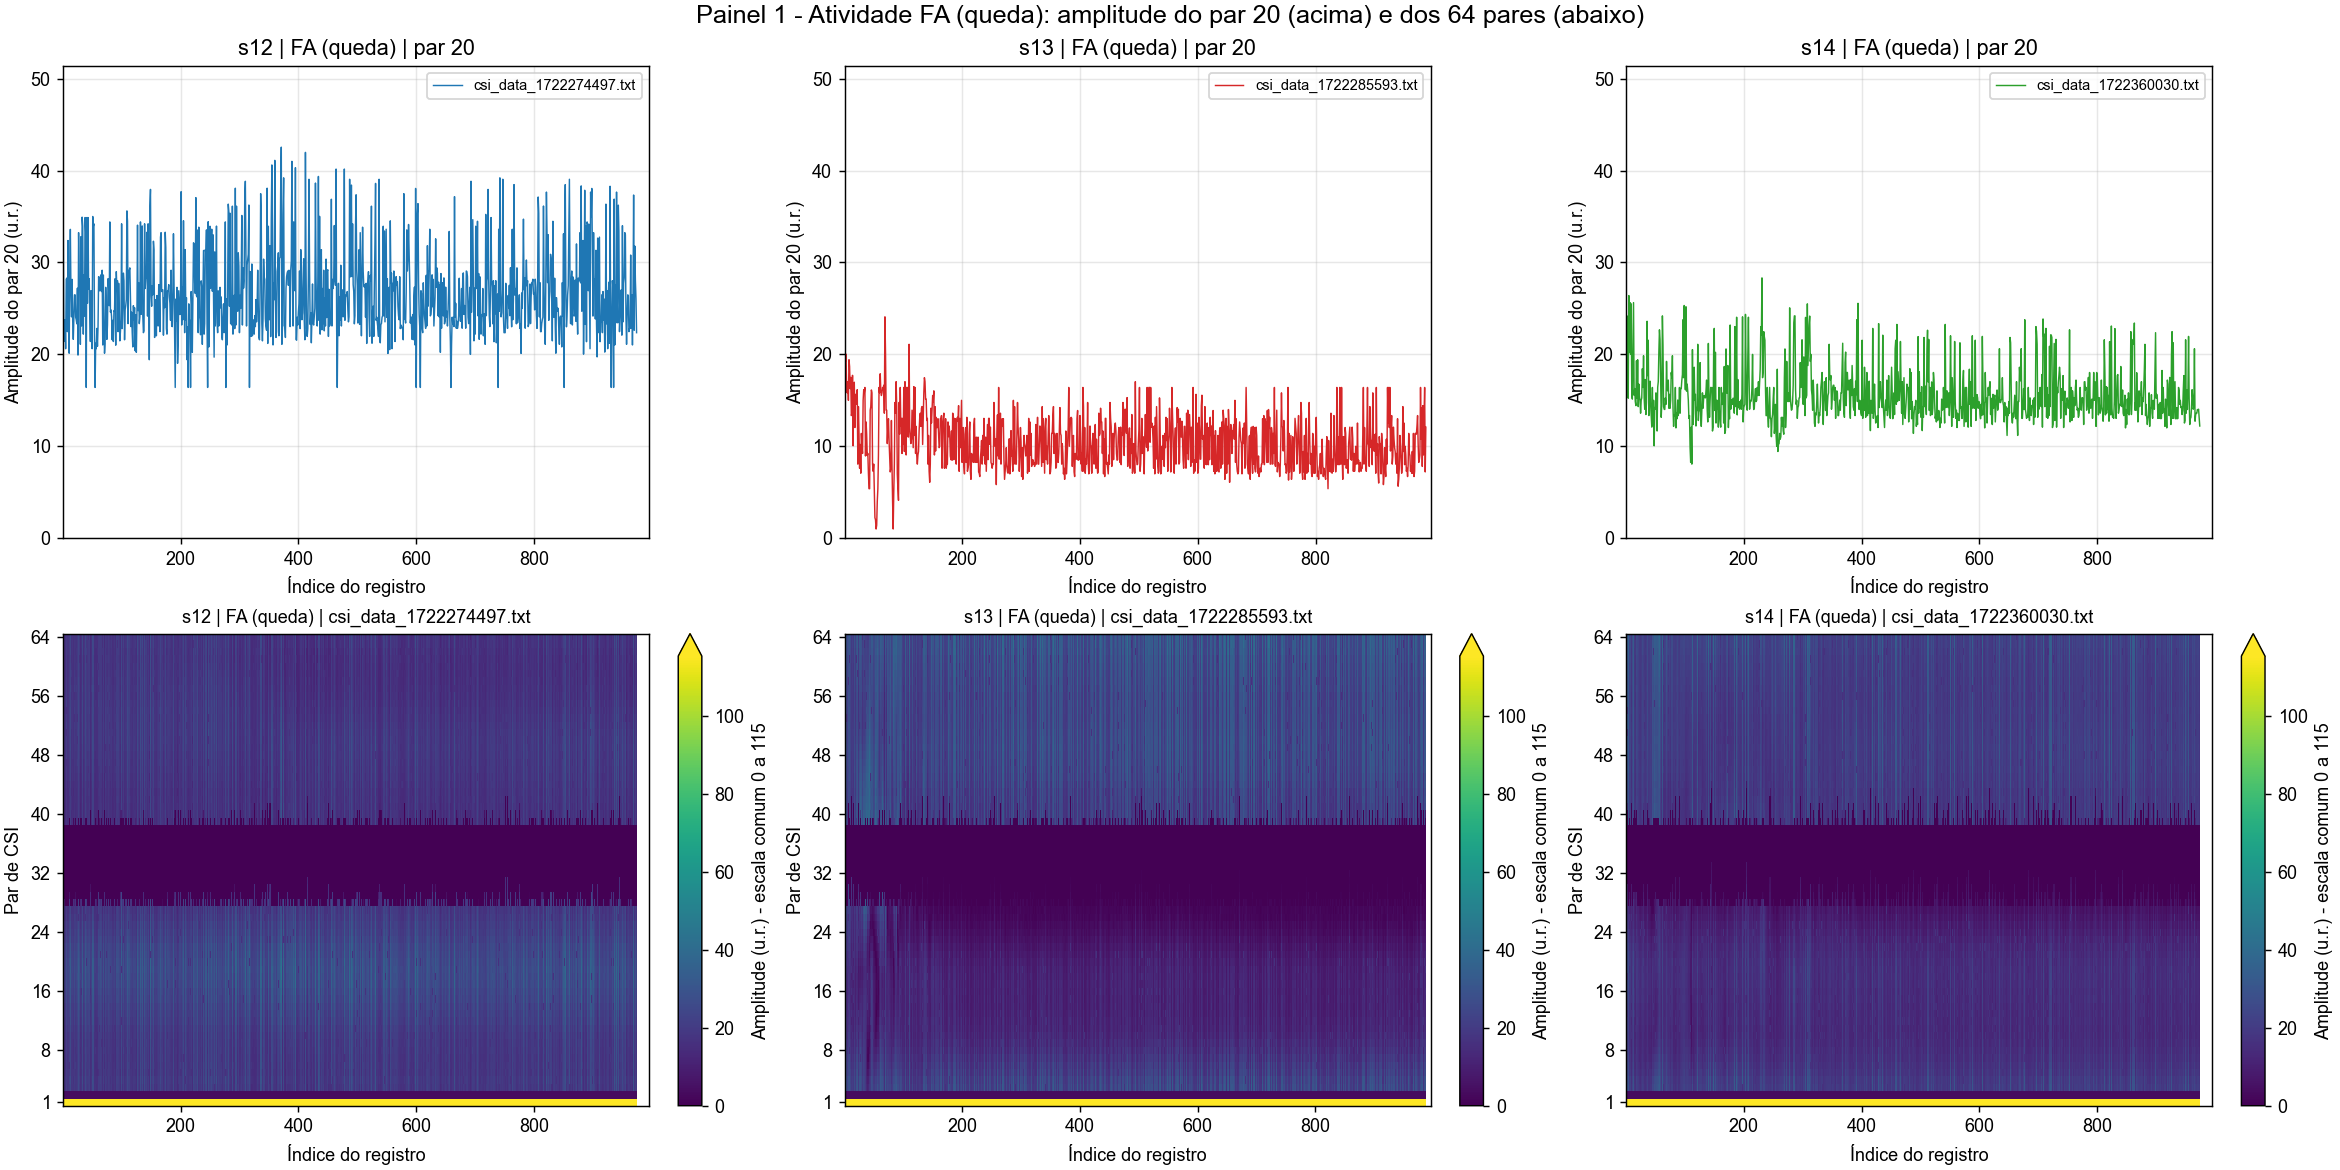
\includegraphics[width=1.00\textwidth,height=19.0cm,keepaspectratio]{Imagens/sec3_painel1_FA.png}
    \caption{Painel 1 - atividade FA (queda): séries temporais do par 20 (acima) e mapas de calor dos 64 pares (abaixo) para s12, s13 e s14 (ordem\_selecao = 1). (arquivo: figuras/sec3\_painel1\_FA.png)}
    \label{fig:sec3_painel1_FA}
\end{figure}

\begin{figure}[H]
    \centering
    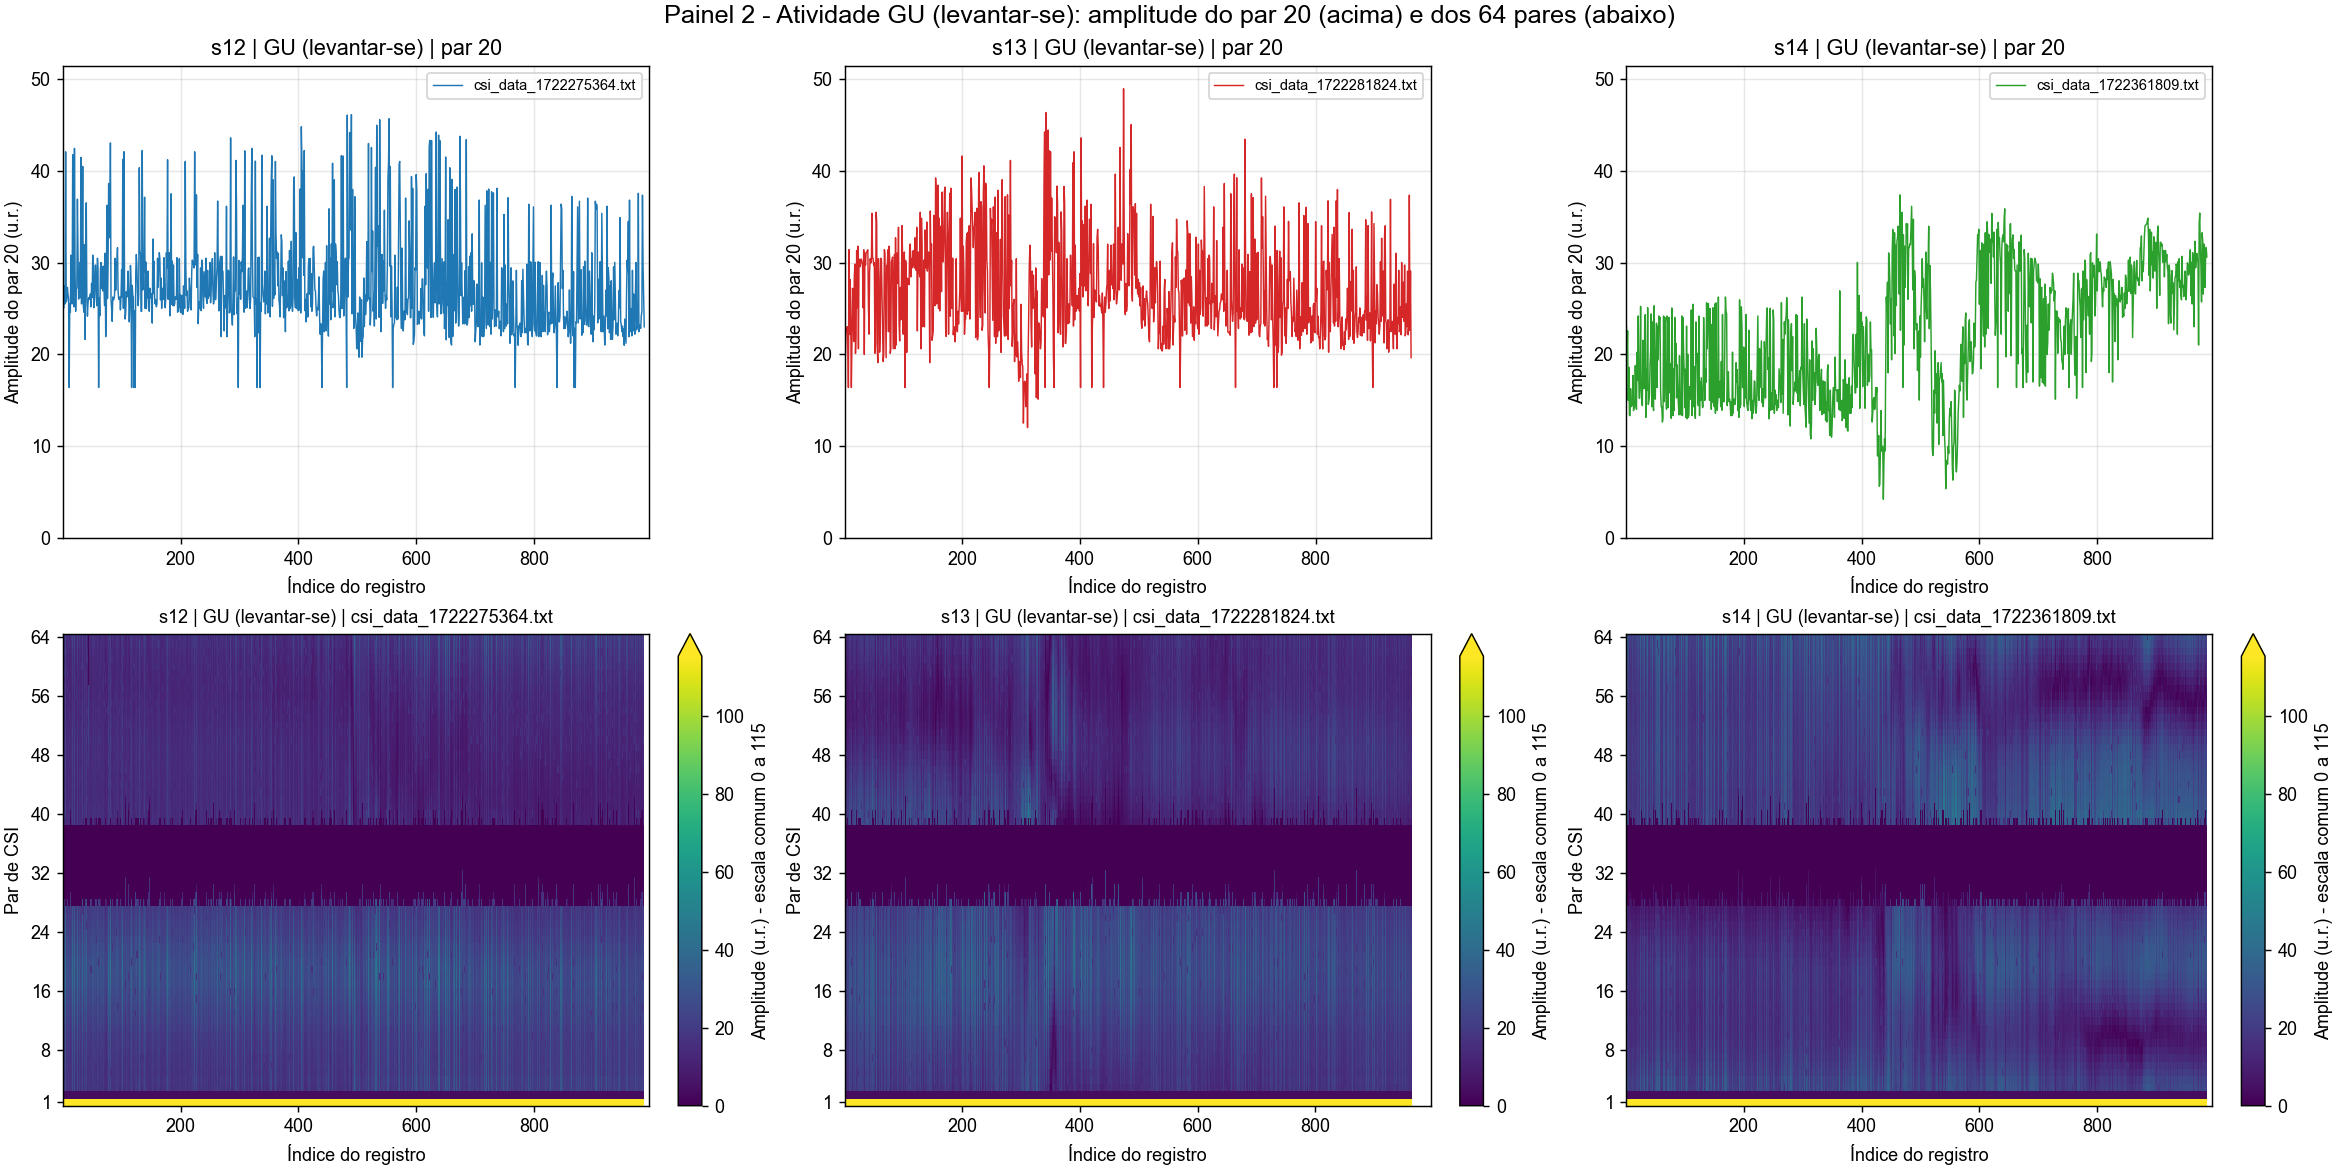
\includegraphics[width=1.00\textwidth,height=19.0cm,keepaspectratio]{Imagens/sec3_painel2_GU.png}
    \caption{Painel 2 - atividade GU (levantar-se): séries temporais do par 20 (acima) e mapas de calor dos 64 pares (abaixo) para s12, s13 e s14 (ordem\_selecao = 1). (arquivo: figuras/sec3\_painel2\_GU.png)}
    \label{fig:sec3_painel2_GU}
\end{figure}

\begin{figure}[H]
    \centering
    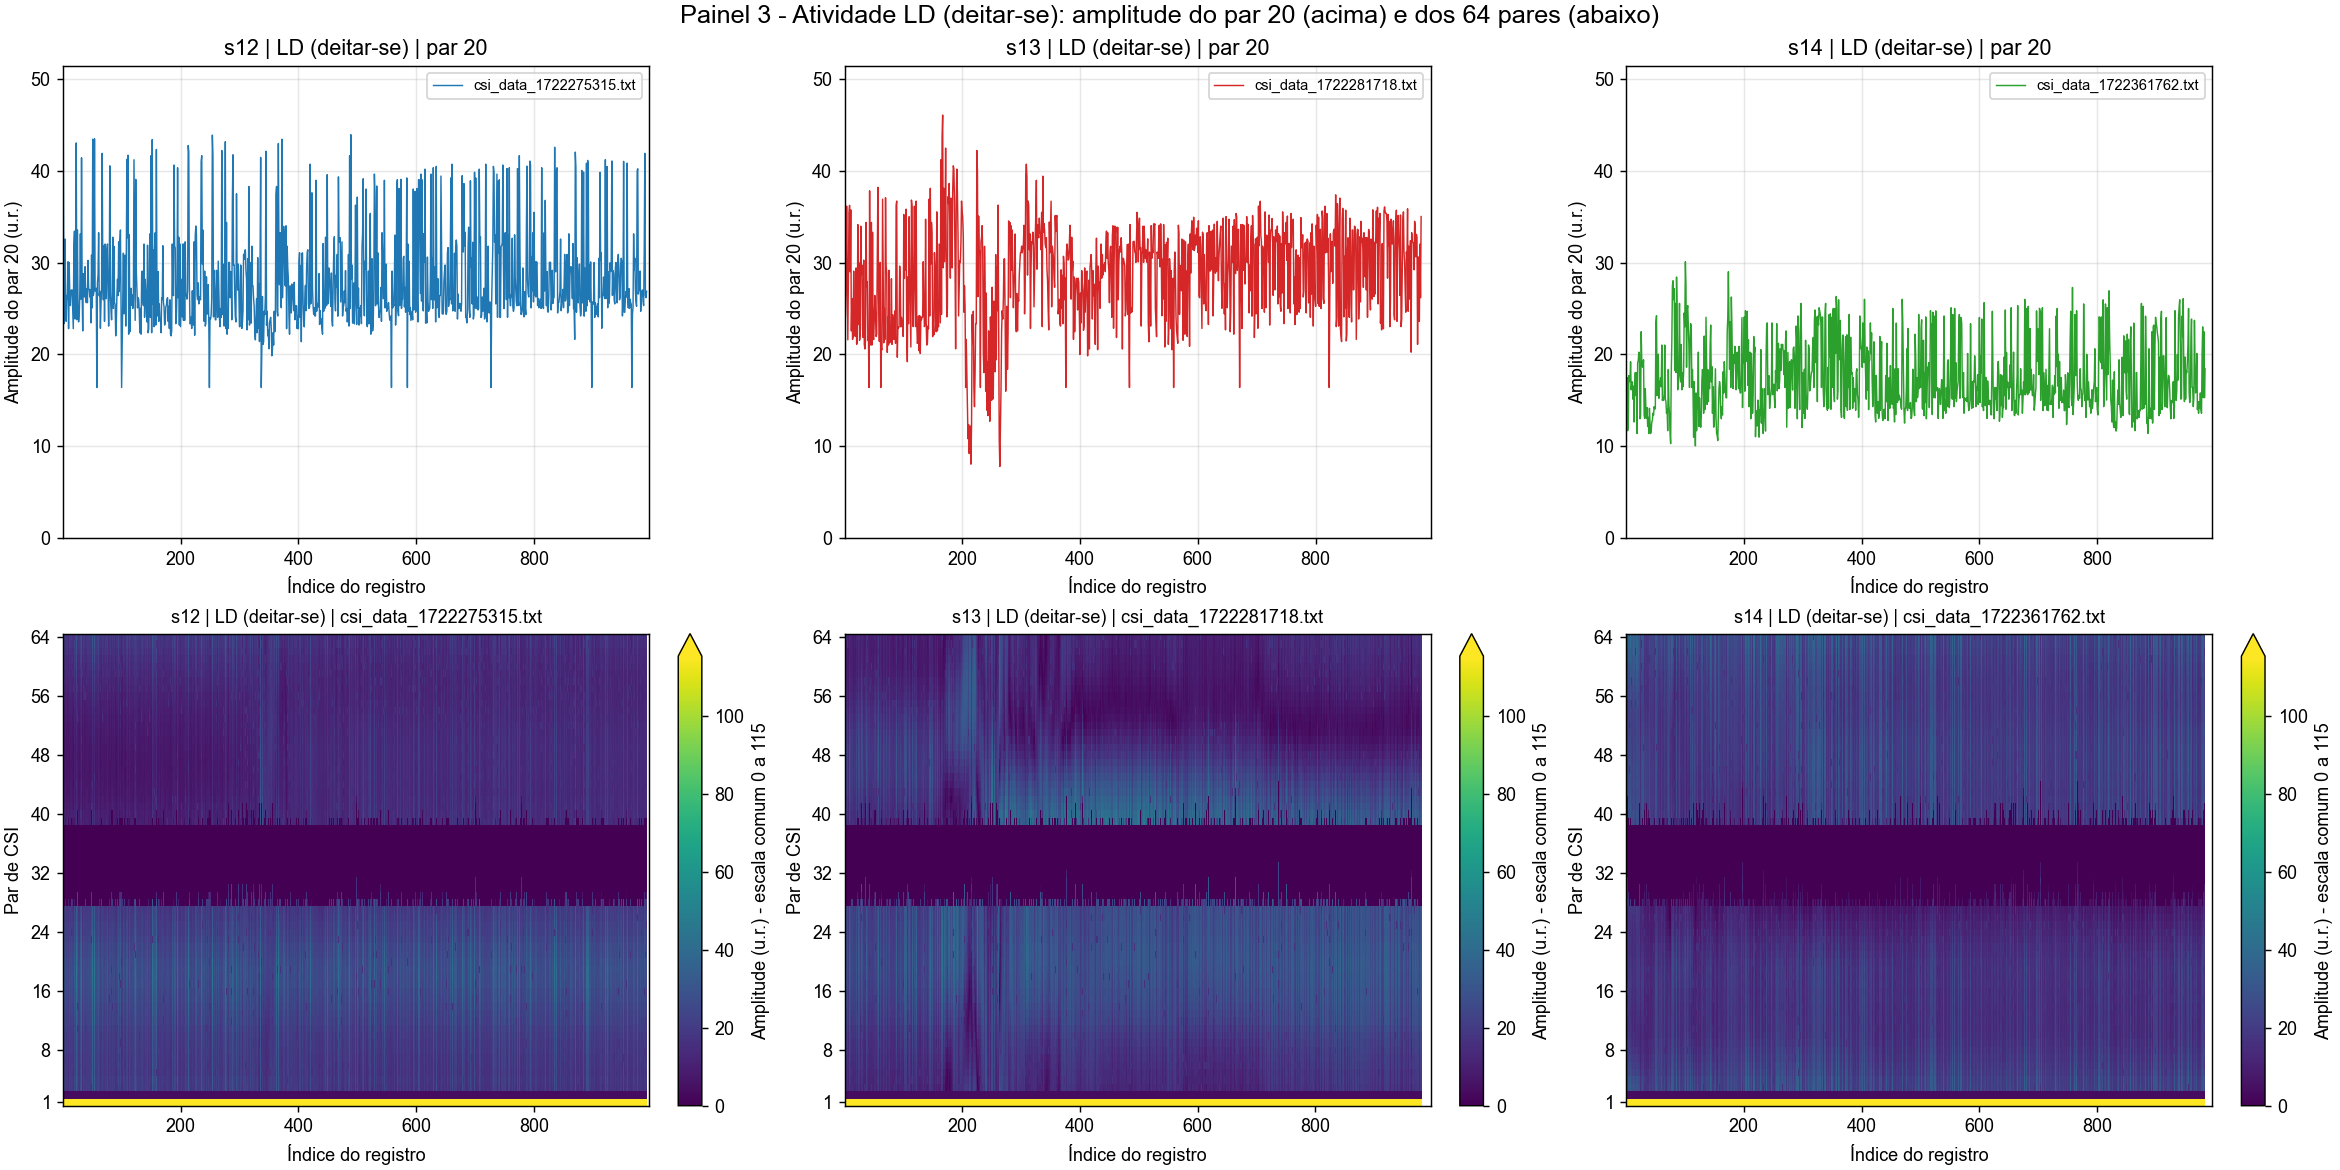
\includegraphics[width=1.00\textwidth,height=19.0cm,keepaspectratio]{Imagens/sec3_painel3_LD.png}
    \caption{Painel 3 - atividade LD (deitar-se): séries temporais do par 20 (acima) e mapas de calor dos 64 pares (abaixo) para s12, s13 e s14 (ordem\_selecao = 1). (arquivo: figuras/sec3\_painel3\_LD.png)}
    \label{fig:sec3_painel3_LD}
\end{figure}

\begin{figure}[H]
    \centering
    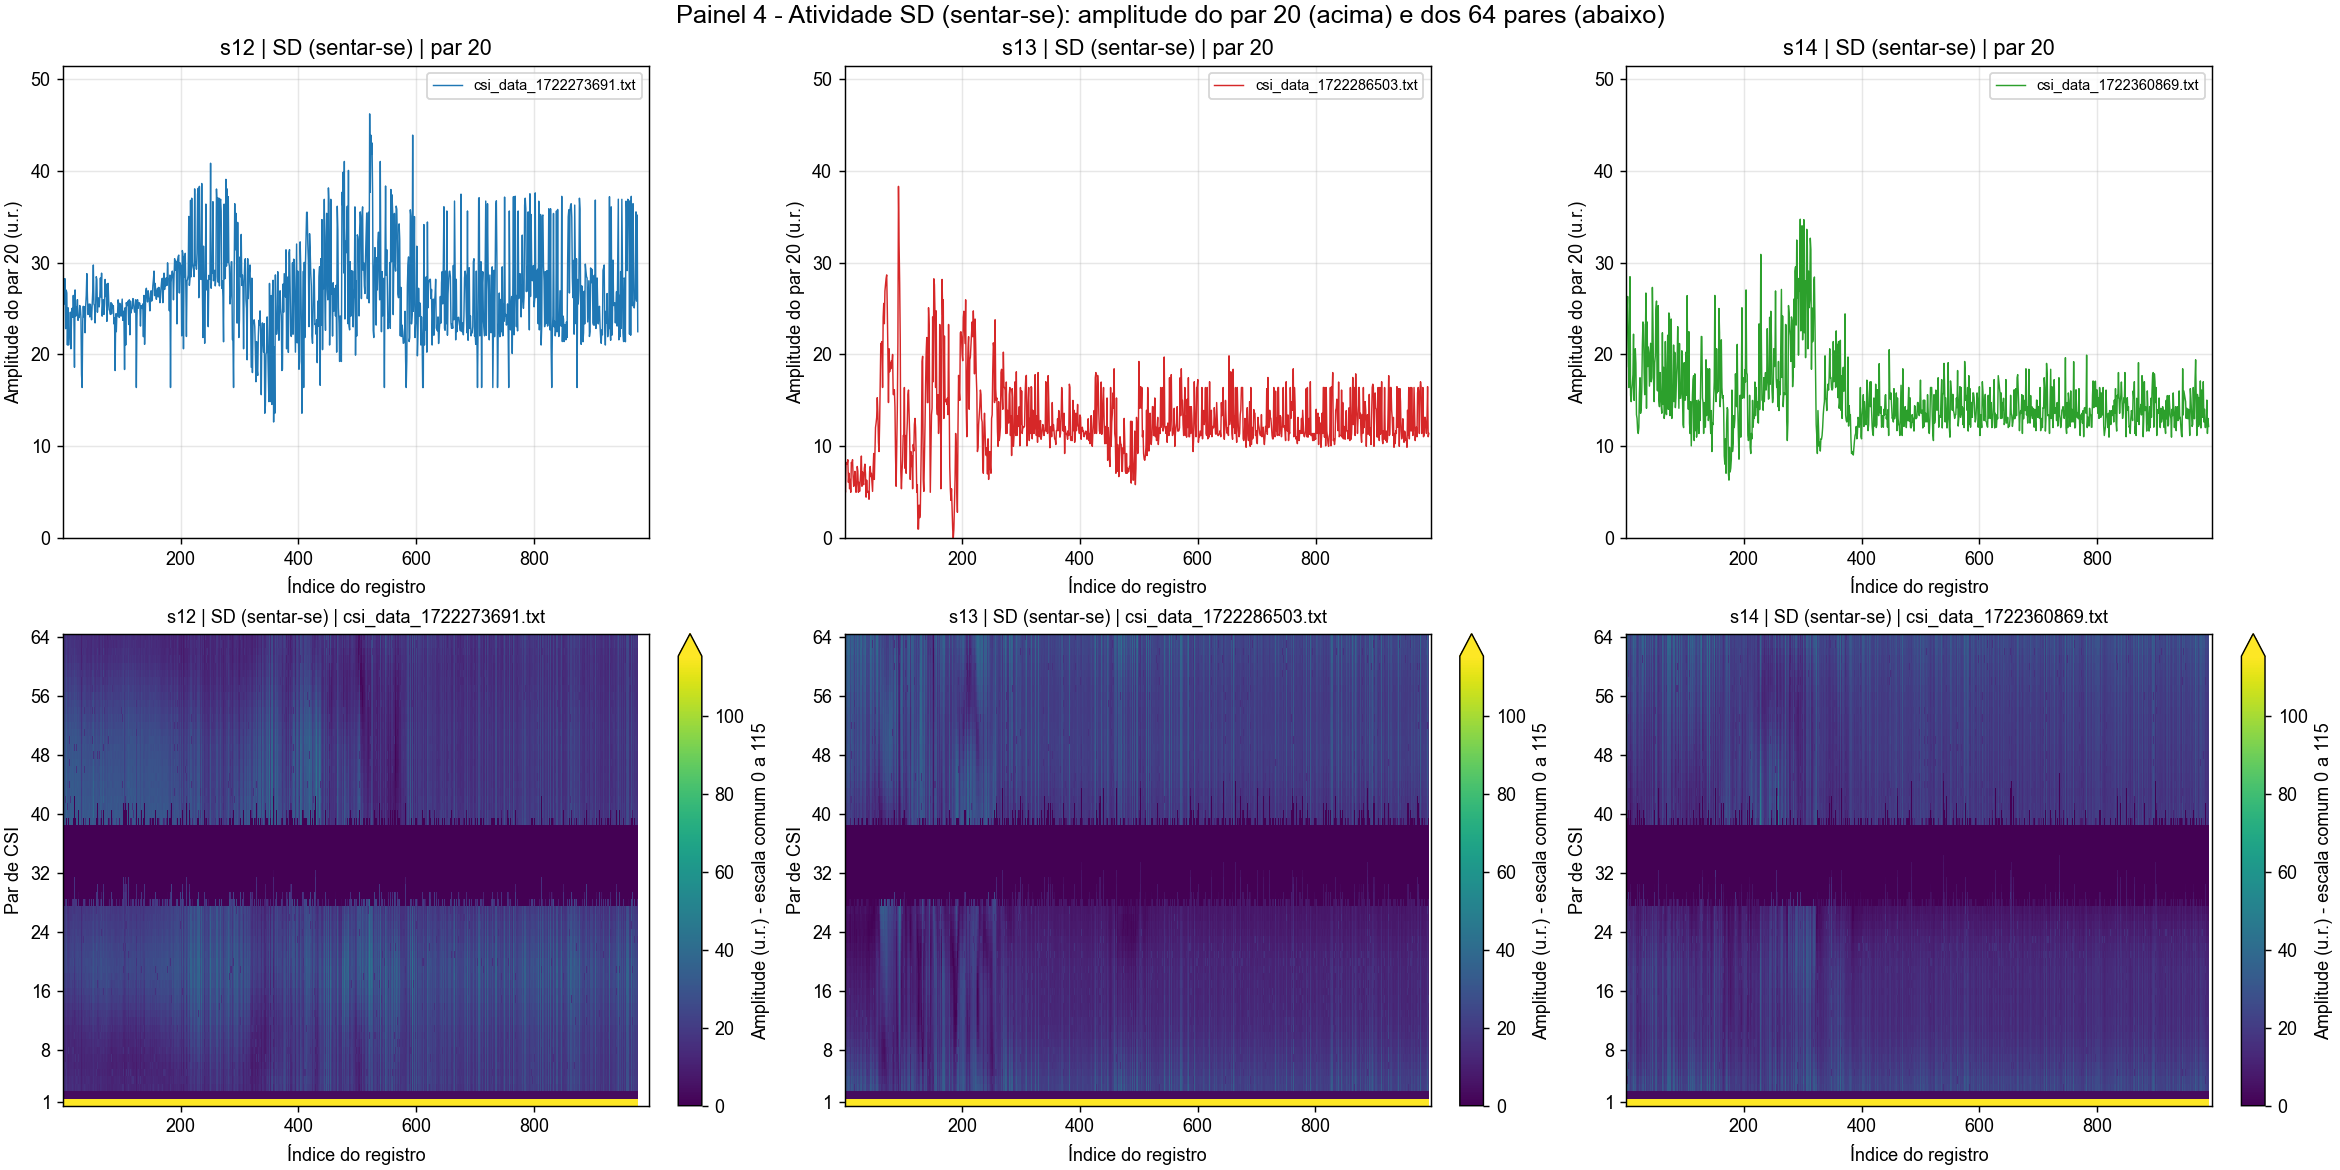
\includegraphics[width=1.00\textwidth,height=19.0cm,keepaspectratio]{Imagens/sec3_painel4_SD.png}
    \caption{Painel 4 - atividade SD (sentar-se): séries temporais do par 20 (acima) e mapas de calor dos 64 pares (abaixo) para s12, s13 e s14 (ordem\_selecao = 1). (arquivo: figuras/sec3\_painel4\_SD.png)}
    \label{fig:sec3_painel4_SD}
\end{figure}

\begin{figure}[H]
    \centering
    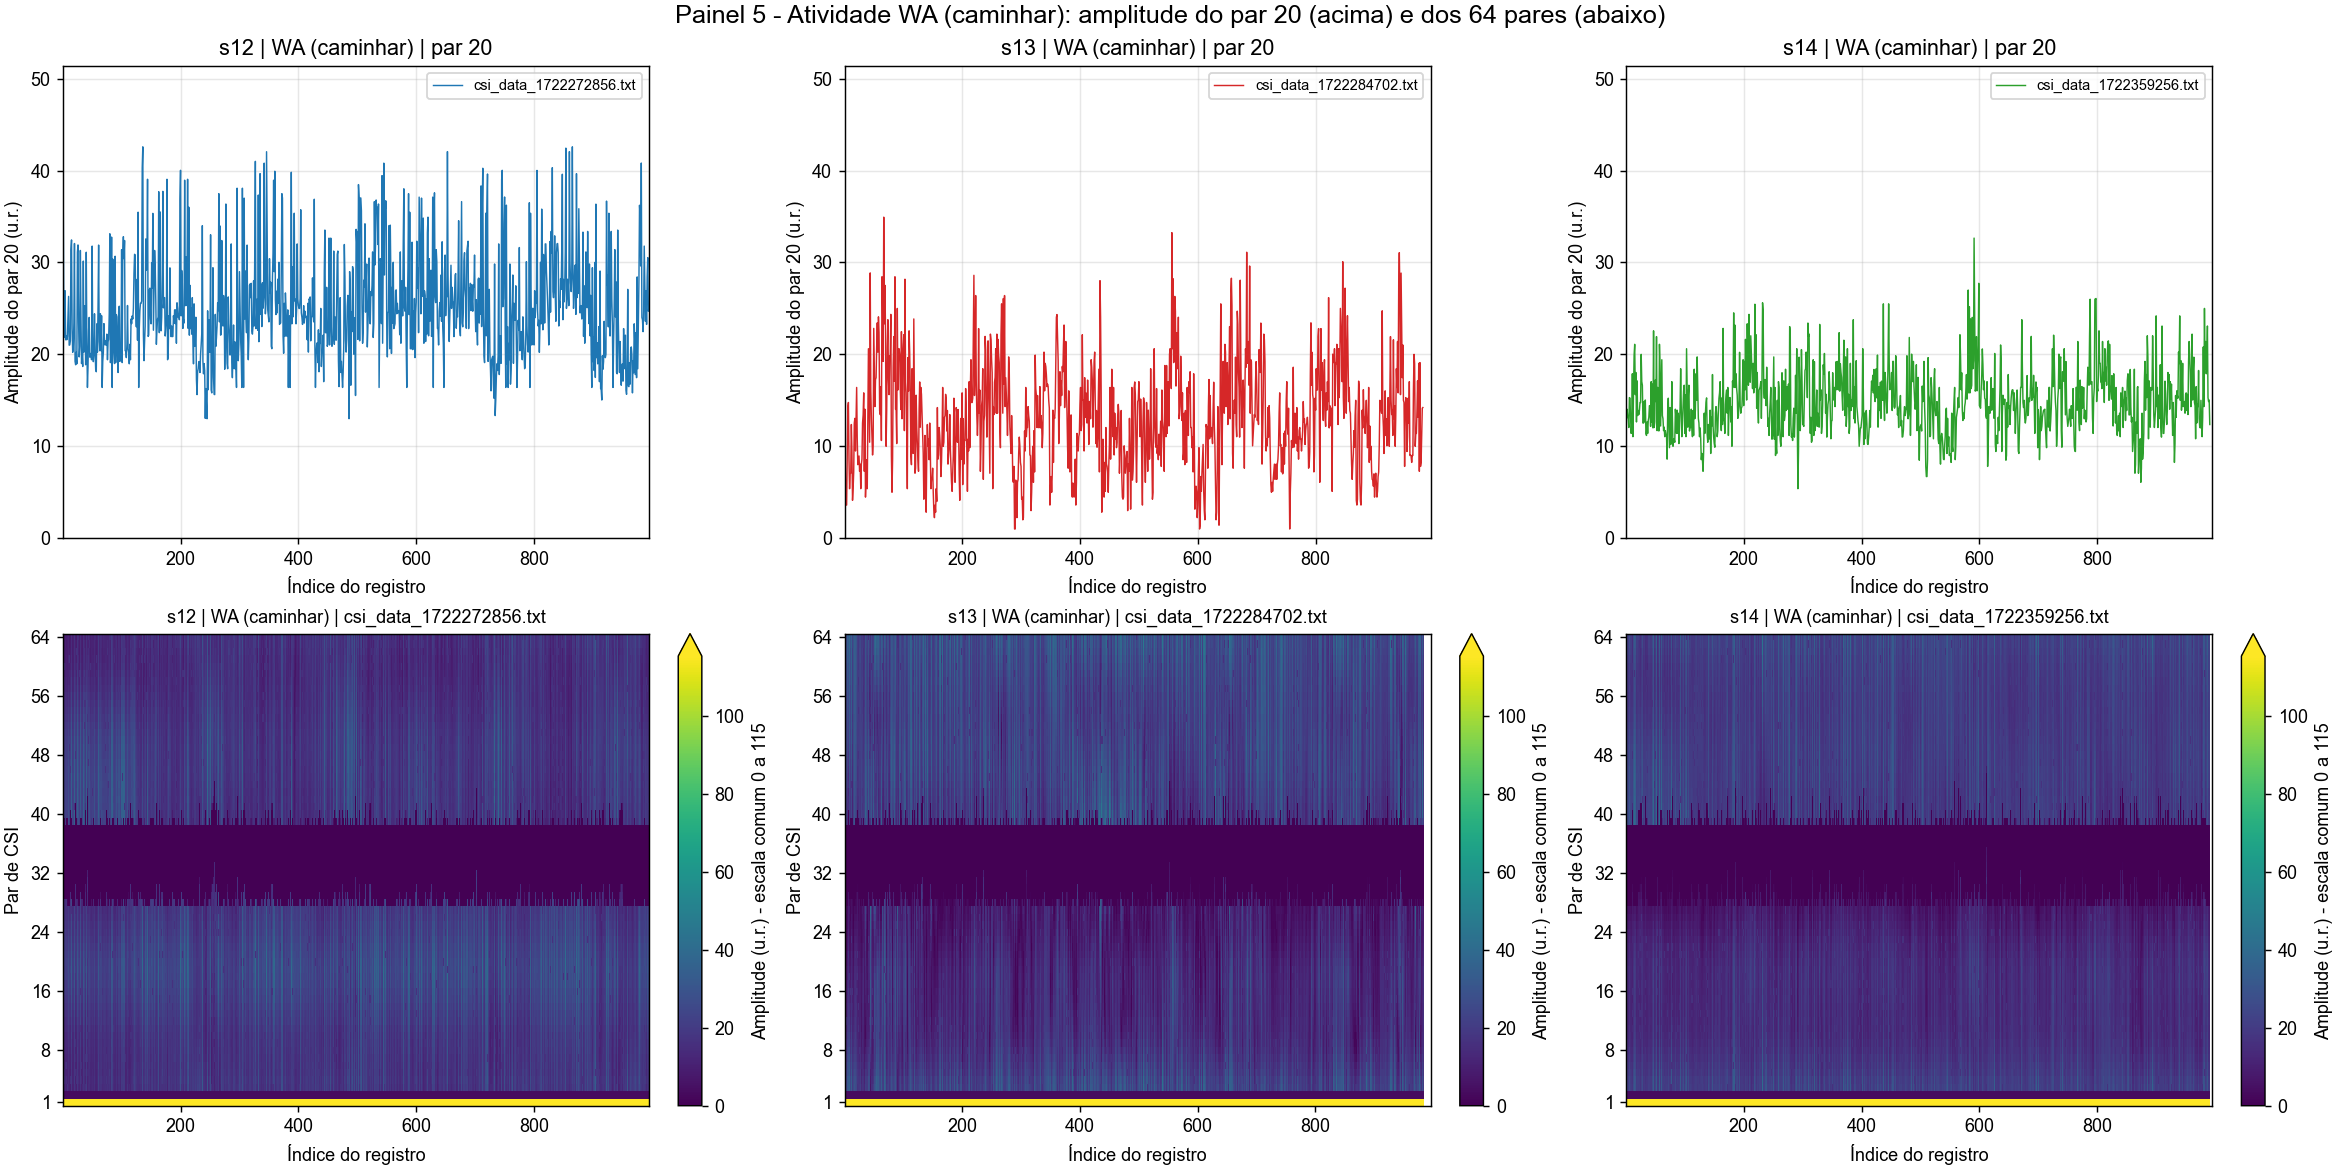
\includegraphics[width=1.00\textwidth,height=19.0cm,keepaspectratio]{Imagens/sec3_painel5_WA.png}
    \caption{Painel 5 - atividade WA (caminhar): séries temporais do par 20 (acima) e mapas de calor dos 64 pares (abaixo) para s12, s13 e s14 (ordem\_selecao = 1). (arquivo: figuras/sec3\_painel5\_WA.png)}
    \label{fig:sec3_painel5_WA}
\end{figure}

\subsection{Interpretação}

\textbf{1. Mesma atividade, pessoas diferentes.} A característica mais evidente é o \textbf{nível} da amplitude do par 20, que difere mais entre participantes do que entre atividades: s12 oscila em torno de 25-28 em todas as atividades, s14 em torno de 15-22, e s13 tem dois níveis (cerca de 10-13 em FA, SD e WA e cerca de 27-29 em GU e LD). Quanto à forma:

\begin{itemize}
    \item \textbf{SD (Figura 4)} é a atividade com maior semelhança entre os três: todos apresentam um trecho inicial perturbado seguido de um trecho estável. Em s13 a perturbação ocupa os registros $\sim$1-250 (desvio padrão por janela de 100 registros de 7,6, 7,1 e 4,7, caindo para $\sim$2 depois do registro 300); em s14, os registros $\sim$1-400 (pico de $\sim$35 perto do registro 300; depois do registro 400 o desvio por janela fica entre 1,7 e 2,0); em s12 a perturbação é mais tardia, registros $\sim$200-600 (queda até $\sim$13 perto do registro 350 e pico de 46 perto do 520).
    \item \textbf{FA (Figura 1)}: s13 e s14 têm maior variação nos primeiros registros (s13: janela 1-100 com desvio 4,9 contra $\sim$2,5 no restante; s14: registros 1-300 com 3,2-3,8 contra $\sim$2,7), enquanto s12 oscila de forma densa e uniforme (20 a 42) em toda a gravação.
    \item \textbf{GU (Figura 2)}: s14 apresenta grandes mudanças de nível - de $\sim$15-25 até o registro $\sim$400, quedas até $\sim$5 perto dos registros 430 e 550 e subida para $\sim$30 depois do registro 600 (desvio de 8,4 na janela 401-500). s13 varia mais nos registros 201-400 (6,6 e 7,6) e s12 é mais uniforme.
    \item \textbf{LD (Figura 3)}: s13 tem uma perturbação marcada nos registros $\sim$150-300 (quedas até $\sim$8 perto dos registros 210 e 260), visível também no mapa de calor como mudança de cor nos pares 40-64 a partir do registro $\sim$350. s12 e s14 são mais uniformes.
    \item \textbf{WA (Figura 5)}: a variação se distribui ao longo de toda a gravação, sem um único trecho dominante. Em s13 aparecem surtos quase periódicos a cada $\sim$100-150 registros, compatíveis com idas e vindas entre os pontos de caminhada, mas sem anotação não é possível confirmar.
\end{itemize}
\textbf{2. Mesma pessoa, atividades diferentes.} Para \textbf{s13}, FA e SD mostram um transiente no início seguido de sinal estável, WA mostra variação durante toda a gravação, e GU/LD têm nível bem mais alto. Para \textbf{s14}, GU tem as maiores mudanças de nível, SD tem o trecho final mais estável de todas as gravações e FA/LD/WA têm variação moderada e contínua. Para \textbf{s12}, as cinco atividades são visualmente parecidas (mesmo nível, oscilação densa entre $\sim$16 e $\sim$45); apenas SD mostra um trecho claramente diferente (registros $\sim$200-600). Em s12 aparece repetidamente o mesmo valor mínimo de 16,4, consequência de os componentes do CSI serem inteiros (as amplitudes assumem valores discretos).

\textbf{3. Variação durante a gravação.} Os trechos de maior variação (desvio por janela de 100 registros, arquivo apoio\_variacao\_janelas\_par20.csv) são: s13/SD registros 1-200 (7,6 e 7,1), s14/GU 401-600 (8,4 e 7,1), s13/GU 301-400 (7,6), s13/LD 201-300 (7,6) e s12/SD 501-600 (6,3). Os de menor variação são os trechos finais de s14/SD (registros 401-989, 1,7-2,0), s13/SD (301-992, 2,0-2,4) e o trecho inicial de s12/SD (1-200, 2,2-2,6), indicando a pessoa parada. Nas atividades de transição (SD, GU, LD, FA) a variação tende a se concentrar em um trecho; em WA ela é distribuída. O instante exato de cada movimento (por exemplo, da queda) não é afirmado, pois a base não tem anotação temporal.

\textbf{4. Comportamento dos pares.} Nos 15 mapas de calor aparecem sempre as mesmas faixas (estatísticas por par em apoio\_estatisticas\_por\_par.csv):

\begin{itemize}
    \item \textbf{Par 1}: amplitude constante de $\sim$115 (desvio médio 0,05) em todas as gravações - faixa amarela na base dos mapas. Por não variar, não carrega informação sobre o movimento.
    \item \textbf{Par 2}: constante em 4,0 (desvio 0).
    \item \textbf{Pares 33 a 38}: amplitude zero (desvio $\leq$ 0,1) - faixa escura central.
    \item \textbf{Pares 28 a 32}: amplitudes decrescentes e próximas de zero (médias 5,2; 1,6; 0,6; 0,2; 0,06).
    \item \textbf{Par 39}: transição, com média 13,7 mas o maior desvio padrão (10,1).
    \item Os pares 3-27 e 40-64 têm amplitudes de $\sim$15-21 e variação de $\sim$4-5. Isso é coerente com a estrutura do canal 802.11n de 20 MHz descrita no artigo (52 subportadoras de dados, 4 piloto e 8 nulas); os autores removem os índices 0 e 27-37 (pares 1 e 28-38) em imf\_generator.py, ficando com 52 pares.
\end{itemize}
\newpage
